\documentclass[a4paper,14pt]{article}
\usepackage[14pt]{extsizes}




\usepackage{cmap}					% поиск в PDF
\usepackage{mathtext} 				% русские буквы в формулах
\usepackage[T2A]{fontenc}			% кодировка
\usepackage[utf8]{inputenc}			% кодировка исходного текста
\usepackage[english,russian]{babel}	% локализация и переносы
\usepackage{ulem}                   % зачеркнутый текст
\usepackage{amssymb}			% пакет математики
\usepackage{float}
\usepackage{amsmath}
\usepackage{graphicx}
\DeclareGraphicsExtensions{.png}

%%% Страница
%\usepackage{extsizes} % Возможность сделать 14-й шрифт
\usepackage[left=1cm,right=1cm,top=1cm,bottom=1cm]{geometry} % Простой способ задавать поля
\pagestyle{empty}

\begin{document}


\begin{center}
ФЕДЕРАЛЬНОЕ ГОСУДАРСТВЕННОЕ ОБРАЗОВАТЕЛЬНОЕ БЮДЖЕТНОЕ УЧРЕЖДЕНИЕ ВЫСШЕГО ОБРАЗОВАНИЯ

    \textbf{«ФИНАНСОВЫЙ УНИВЕРСИТЕТ ПРИ ПРАВИТЕЛЬСТВЕ РОССИЙСКОЙ ФЕДЕРАЦИИ»}

Факультет информационных технологий и анализа больших данных

Департамент анализа данных и машинного обучения

\textit{
	\textbf{Дисциплина: «Теория вероятностей и математическая статистика»}}

\textit{Направление подготовки: 01.03.02 «Прикладная математика и информатика»}

\textit{Профиль: «Анализ данных и принятие решений в экономике и финансах»}

\textit{Форма обучения очная, учебный 2020/2021 год, 4 семестр}

\textbf{Билет 116}

\end{center}

\begin{enumerate}


\item


Дайте определение случайной величины, которая имеет $\chi ^{2}$-распределение с n степенями свободы.
Запишите плотность $\chi ^{2}$- распределения. Выведите формулы для математического ожидания $\mathbb{E}(X)$ и дисперсии $\mathbb{V}ar(X)$ $\chi ^{2}$-распределение с n степенями свободы. Найдите а) $\mathbb{P}(\chi _{20}^{2} > 10.9)$, где $\chi _{20}^{2}$–случайная величина, которая имеет $\chi ^{2}$– распределение с 20 степенями свободы; б) найдите 93\%
(верхнюю) точку $\chi _{0.93}^{2} (5)$ хи-квадрат распределения с 5 степенями свободы




$\mathbb{P}(\chi _{20}^{2} > 10.9) =  0.948775$; $\chi _{0.93}^{2} (5) = 1.34721$.


\item



Случайные величины $X$ и $Y$ независимы и имеют равномерное
распределение на отрезках $[0;7]$ и $[0;3]$ соответственно. Для случайной величины $Z=\frac{Y}{X}$ найдите: 
1) функцию распределения $F_Z(x)$;
2) плотность распределения $f_Z(x)$ и постройте график плотности;
3) вероятность $\P(0,\!006\leqslant Z\leqslant 0,\!519)$.




%\folder 2_53d18.png
1) Функция распределения $F_Z(x)$ имеет вид:
$
F_Z(x)=\left\{
\begin{array}{l}
0, x\leqslant 0;\\
\frac{7 x}{6}, 0\leqslant x\leqslant \frac{3}{7}\approx 0,\!429;\\
1 - \frac{3}{14 x}, x\geqslant\frac{3}{7};
\end{array}.
\right.
$
2) Плотность распределения $f_Z(x)$ имеет вид:
$
f_Z(x)=\left\{
\begin{array}{l}
0, x<0;\\
\frac{7}{6}, 0\leqslant x\leqslant \frac{3}{7}\approx 0,\!429;\\
\frac{3}{14 x^{2}}, x\geqslant\frac{3}{7};
\end{array}.
\right.
$


\begin{figure}[H]
    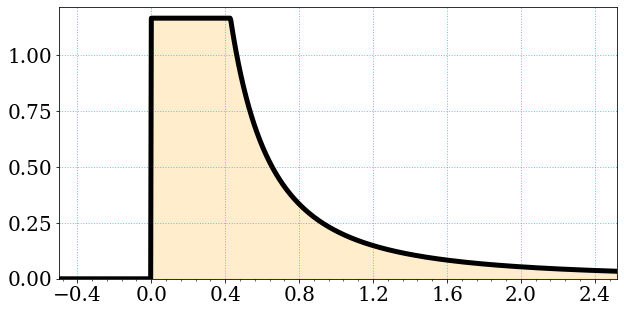
\includegraphics[width=0.9\textwidth]{2_53d18}
\end{figure}


3) вероятность равна:
$
\P(0,\!006\leqslant Z\leqslant 0,\!519)=
0,\!57962.
$


\item

    
	Случайная величина Y принимает только значения из множества $\{3, 4\}$, при этом $P(Y=3) = 0.33$.
	Распределение случайной величины X определено следующим образом:
	\begin{equation*}
		X | Y =
		\begin{cases}
			$9$ * y, с вероятностью $ 0.34$ \\
			$7$ * y, с вероятностью $ 1 - 0.34$
		\end{cases}
	\end{equation*}

	Юный аналитик Дарья нашла матожидание и дисперсию $X$.

	Помогите Дарье найти матожидание и дисперсию величины $X$
	


	

	Первым этапом надо найти характеристики случайной величины $Y$

	$E(Y) = 3 * 0.33 + 4 * (1 - 0.33)$

	$Var(Y) = E(Y^2) - [E(Y)]^2 = 3^2 * 0.33 + 4^2 * (1 - 0.33) - [E(Y)]^2$


	Перейдем к рассмотрению характеристик условной случайно величины X

	$E(X) = E(E(X|Y)) = E[E(9 * Y) * 0.34 + E(7 * Y) * (1 - 0.34)] = E(Y) * (9 * 0.34 + 7 * (1 - 0.34)) = 28.1856$

	$E(Var(X|Y)) = E[b * Var(c3 * Y) + (1 - b) * Var(c4 * Y)] = Var(Y) * (c3^2 * b + c4^2 * (1- b)) $

	$Var(E(X|Y)) = E(X^2|Y) - [E(X)]^2 = [E(Y)]^2 * (b * c3^2 + (1-b)*c4^2) - E(X)]^2$

	$Var(X) = E(Var(X|Y)) + Var(E(X|Y)) = 25.32915$
	

\item


(10) В группе $\Omega$ учатся студенты:$\omega _{1}...\omega _{25}$ . Пусть $X$ и $Y$ – 100-балльные экзаменационные оценки по
математическому анализу и теории вероятностей. Оценки $\omega _{i}$ студента обозначаются: $x _{i} = X(\omega _{i})$ и $y _{i} = Y(\omega _{i})$, $i = 1...25$. Все оценки известны
$x _{0} = 55, y _{0} = 54$, $x _{1} = 64, y _{1} = 68$, $x _{2} = 34, y _{2} = 51$, $x _{3} = 48, y _{3} = 73$, $x _{4} = 81, y _{4} = 69$, $x _{5} = 62, y _{5} = 69$, $x _{6} = 76, y _{6} = 59$, $x _{7} = 84, y _{7} = 45$, $x _{8} = 97, y _{8} = 77$, $x _{9} = 76, y _{9} = 87$, $x _{10} = 43, y _{10} = 67$, $x _{11} = 33, y _{11} = 55$, $x _{12} = 71, y _{12} = 96$, $x _{13} = 62, y _{13} = 97$, $x _{14} = 84, y _{14} = 37$, $x _{15} = 41, y _{15} = 70$, $x _{16} = 92, y _{16} = 41$, $x _{17} = 60, y _{17} = 54$, $x _{18} = 71, y _{18} = 44$, $x _{19} = 39, y _{19} = 70$, $x _{20} = 98, y _{20} = 75$, $x _{21} = 99, y _{21} = 32$, $x _{22} = 58, y _{22} = 42$, $x _{23} = 61, y _{23} = 92$, $x _{24} = 58, y _{24} = 32$
Требуется
найти следующие условные эмпирические характеристики: 1) ковариацию $X$ и $Y$ при условии, что одновременно $X \geqslant 50$
 и $Y \geqslant 50$; 2) коэффициент корреляции $X$ и $Y$ при том же условии.




1) Ковариация = $276.75$
2) Коэффициент корреляции = $1.373$


\item


(10) Эмпирическое распределение признаков $X$ и $Y$ на генеральной совокупности $\Omega$ задано таблицей частот  
 
\begin{tabular}{ | c | c | c | c | }
\hline
 & $Y = 2$ & $Y = 4$ & $Y = 5$  \\ \hline
$X = 200$ & $1$ & $18$ & $12$\\ \hline
$X = 300$ & $31$ & $26$ & $12$\\
\hline
\end{tabular}

Из $\Omega$ случайным образом без возвращения извлекаются $12$ элементов. 
Пусть $\bar X$ и $\bar Y$ – средние значения признаков на выбранных элементах. 
Требуется найти: 1) математическое ожидание $\mathbb{E}(\bar Y)$; 2) стандартное отклонение $\sigma(\bar X)$ ; 
3) ковариацию $Cov(\bar X, \bar Y)$




1) математическое ожидание $\mathbb{E}(\bar Y)$: $3.6$ 
2) стандартное отклонение $\sigma(\bar X)$: $256.084$
3) ковариацию $Cov(\bar X, \bar Y)$: $-1.9911$


\item


(10) Пусть $X _{1}$, $X _{2}$, $X _{3}$, $X _{4}$ выборка из $N(\theta, \sigma ^{2})$. Рассмотрим две оценки параметра $\theta$:
\[\hat \theta _{1} = \frac{X _{1} + 6X _{2} + X _{3} + 2X _{4}}{10}, \hat \theta _{1} = \frac{3X _{1} + X _{2} + 3X _{3} + 3X _{4}}{10}\]
a) Покажите, что обе оценки несмещенные.
б) Какая из оценок оптимальная?




Обе они несмещенные, потому что в числителе выходит в сумме 10.
Какая-то точно должна быть, а может и нет....


\end{enumerate}

\begin{figure}[H]
	Подготовил
	\hfill
	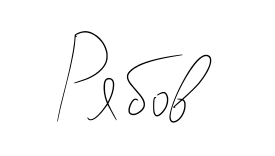
\includegraphics[width=2cm]{Prepared}
	П.Е. Рябов
\end{figure}


\begin{figure}[H]
	Утверждаю:\\
	Первый заместитель\\
	руководителя департамента\\
	Дата 01.06.2021
	\hfill
	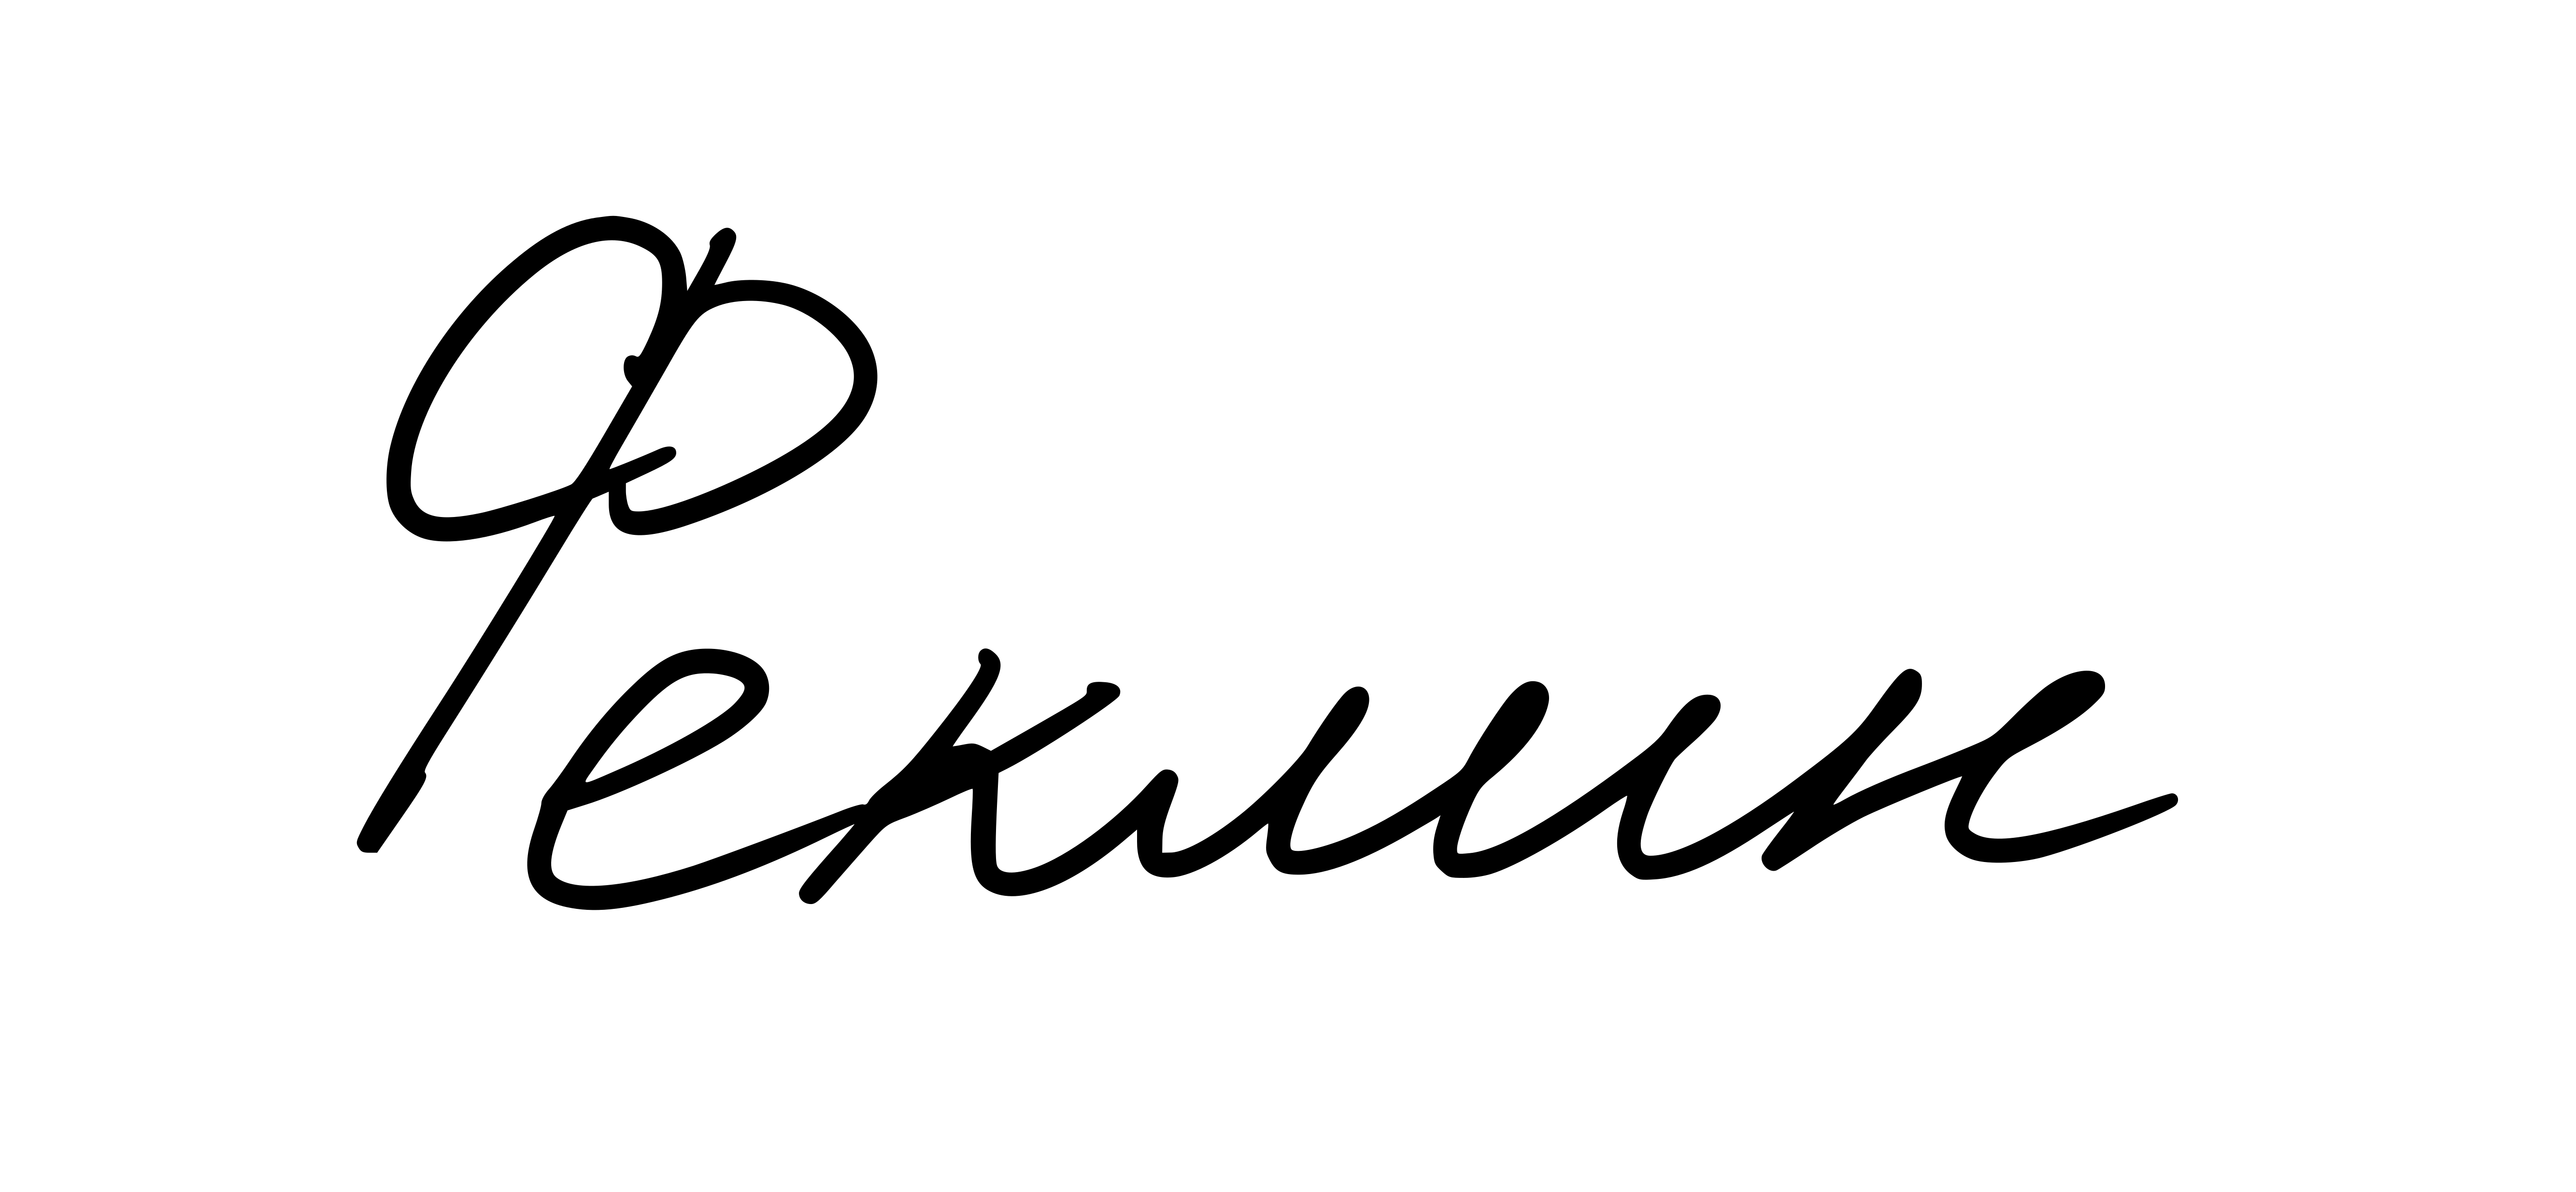
\includegraphics[width=2cm]{Approved}
	Феклин В.Г.
\end{figure}

\end{document}

